% This is main.tex, a sample paper demonstrating the use of the
% LLNCS macro package for Springer Computer Science proceedings;
% Version 2.20 of 2017/10/04
% 
\documentclass[runningheads]{llncs}
%
% ---- Packages ----
%
\usepackage{graphicx} % enhanced support for graphics
\usepackage[obeyspaces]{xurl} % add macros for handling URLs in text
\usepackage[nohyperlinks,nolist]{acronym} % abbreviation utilities
\usepackage{listings}
\usepackage{float}
\usepackage{ntheorem}
\usepackage{amssymb}
\usepackage{footmisc}
\usepackage{footnote}
\usepackage{fourier}
\usepackage{caption}
\usepackage{longtable}
\usepackage[pdfusetitle]{hyperref}

\usepackage[
    type={CC},
    modifier={by},
    version={4.0},
]{doclicense}

\renewcommand{\texttt}[1]{{\renewcommand\UrlFont{\ttfamily}\nolinkurl{#1}}}

% \theoremseparator{:}
% \theorempreskip{1em}
\newtheorem{hypothesis}{Hypothesis}
\renewcommand{\thehypothesis}{H\arabic{hypothesis}}

\setlength{\tabcolsep}{3pt}
\setlength{\textfloatsep}{0.1cm}

% From https://tex.stackexchange.com/questions/192994/writing-roman-numbers-in-equation
\newcommand{\RN}[1]{%
  $\textup{\uppercase\expandafter{\romannumeral#1}}$%
}

\captionsetup[table]{skip=10pt}

% TODO: add more packages below if necessary
%
% ---- Acronyms ----
%
\begin{acronym}
\acro{rq}[RQ]{Research Question}
\acro{rts}[RTS]{Regression Test Selection}
\acro{tap}[TAP]{Test Automation Platform}
\acro{poc}[PoC]{Proof of Concept}
\acro{di}[DI]{Dependency Injection}
\end{acronym}

% 
% ---- Begin Document ----
%
\begin{document}
%
\title{The Unsafety in Java Regression Test Selection and its Occurrence in the Wild}
%
\titlerunning{The Unsafety in Java RTS and Its Occurrence in the Wild}
% If the paper title is too long for the running head, you can set
% an abbreviated paper title here
%
% ---- Author Information ----
%
\author{Lukas Döllerer}
\institute{Seminar: Software Quality\\
  Technical University of Munich\\
  \email{lukas.doellerer@tum.de}}
%
\maketitle % typeset the header of the contribution
%
% ---- Abstract ----
%
\begin{abstract}
  Regression testing is used by developers to ensure that new
  revisions of a program do not negatively impact existing features.
  \ac{rts} excludes test cases from the regression test set. An \ac{rts}-tool that correctly
  selects all tests affected by introduced changes is
  called \emph{safe}. Prior research has shown that this safety is hard to achieve.
  Undetected unsafety can be caused by a faulty implementation or imperfect
  methodology of an \ac{rts}-tool. In this study, we collected known and discovered new unsafety
  in the popular open source \ac{rts}-tools \emph{Ekstazi}, \emph{GIBstazi}, \emph{OpenClover}, \emph{STARTS} and \emph{HyRTS}.
  We compared the tools with each other, based on reference projects that simulate sources of unsafety.
  To confirm the relevance of the discovered unsafety, we performed a broad analysis of its occurrence on a
  selection of the 100 most popular Java
  repositories on the GitHub platform. We were able to document 10 hypothetical scenarios that cause unsafe
  behavior of the examined \ac{rts}-tools. These scenarios include reflections, dependency injection, problems with runtime instrumentation
  and external files. All examined tools acted unsafe. Sources of unsafety were
  found in 88 out of the 100 scanned repositories. This leads us to the conclusion that none of the
  examined tools are currently ready to be safely used in production environments. Further research must combine
  existing knowledge and tools to develop and maintain an up-to-date implementation of \ac{rts} for Java.
  \keywords{Regression Test Selection \and Unsafety \and Java}
\end{abstract}
%
% ---- Text Parts ----
%
\section{Introduction}\label{sec:intro}

% What points should be in here?
% - Why should we care about Regression tests?
%   -> Regressions errors -> Open source -> Evolution
% - What is RTS and why is it required / important
%   -> less testing time -> more frequent testing possible and more immanent feedback for commiters
%   -> less ressources required for testing -> money
% - Approaches to reduce RT-Cost:
%     * Selection -> for multiple runs
%     * Reduction -> reducing test suits by eliminating redundant tests
%     * Prioritization -> Sorting test cases by probability of uncovering faults 

With agile and iterative software development processes, 
project owners need to ensure that every new revision of their program's source code still
complies with the project's specification. They need to make sure that no new bugs were
introduced. Ensuring the project's ongoing compliance is
increasingly complicated due to large, distributed code bases, the involvement of multiple developers and 
complex program
structures. Regression testing is widely used to detect such regression faults by
re-running existing tests to ensure that the 
new code changes have no negative impact on the code base.\cite{rt_in_agile,rt_iterative}

Executing all tests from a project's regression test suite is a time consuming task that also goes
with an economical cost. Even for companies with enormous computing resources, rerunning all
regression tests does not scale well. Google's \ac{tap} deals with an average program delivery frequency of one commit per
second, resulting in 150 million test runs a day~\cite{7965447}.

% This increase in maintenance is also the main 
% factors keeping
% project owners from utilizing automated testing in their projects.\cite{10.1155/2010/620836}
Regression Test Minimization, Regression Test Prioritization and \acf{rts} are the three major approaches
identified by Yoo and Harman (2012) to reduce the computational cost of regression testing~\cite{regression_testing_reduction}. 

% Short introduction to RTS, more than just the naming of the word
\ac{rts} aims to reduce the amount of
unnecessarily executed tests, i.e.~it excludes tests from the test suite whose outcome should not be
affected by the changes. This selection process is based on information about changes in the
program files and source code dependencies of tests cases. Only tests running changed code paths
are selected for execution. Other test cases should not change their behavior with the new code base.

\ac{rts}-tools exist in many variations. Though, one common goal of all examined tools is to be \emph{safe}.
% The test case dependency information can either be
% collected by \emph{statically} analyzing the program's source
% code or by executing the tests and \emph{dynamically} collecting coverage information. This
% information can be collected in different resolutions: Depending on the
% implementation, the test dependencies are collected per module or package, per file, class or method
% or in even smaller logical blocks, at a basic block or statement-level resolution~\cite{rts_techniques}.
An \ac{rts} system which does not exclude tests that can be affected by the applied changes is called
\emph{safe}~\cite{safe_definition}. Any undetected changes to dependencies of tests makes the \ac{rts}-tool \emph{unsafe},
as they open the possibility for regression faults to be overlooked by not running the corresponding
test cases~\cite{rts_techniques}.

Safety is hard to proof. Although many \ac{rts}-tools claim to be safe in most cases, this safety is
often only shown in experimental
evidence~\cite{unsafety_eval,gibstazi_paper} or in comparison to other \ac{rts}-tools~\cite{prestarts,starts_paper,gibstazi_paper}. Unsafety can be caused by methodological
limitations, errors in the implementation of the tool or outdated \ac{rts} software that is no
longer compatible with up-to-date library or language versions.\cite{unsafety_eval} Even if the \ac{rts}-tool's
methodology and implementation is proven to be safe in theory, unsafety can still occur through
third party language extensions such as the Spring Framework. 

With this seminar paper, we provide further insights into the unsafety of the following
open source \ac{rts}-tools for the Java programming language: The dynamic tools
\emph{Ekstazi}~\cite{ekstazimain,ekstazi_tool}, \emph{GIBstazi}~\cite{gibstazi_paper,gibstazi_tool},
\emph{OpenClover}~\cite{openclover_tool} and \emph{HyRTS}~\cite{hyrts_paper,hyrts_tool}, and
the static tool \emph{STARTS}~\cite{starts_paper,starts_tool}.

The last years show a shift in the open source software community away from the examined
\ac{rts}-tools, leading to an abandonment of their code bases. 
Even the often showcased~\cite{hyrts_paper,ekstazispec,ekstazimain} 
projects Apache CXF~\cite{cxf}, Commons Math~\cite{commonsmath}
and Camel~\cite{camel} stop integrating \emph{Ekstazi} into their testing process.\footnote{The
plugin was removed from Apache Camel with commit eb60743f22c2. Apache CXF and Commons Math do not
document a process that involves Ekstazi and did not update the plugin since its introduction in 2014.}

We show the potential and problems of the examined \ac{rts}-tools to help project owners
mitigate the risks and advantages of using \ac{rts} in their quality control procedures.
% In the first part of the study, we take a closer look at the
% examined \ac{rts}-tools in order to discover previously undocumented or unknown sources of unsafety.
% We searched for anomalies in the tools' source codes and problems originating from their general
% methodology. The resulting sources of unsafe behavior where then combined with already documented
% cases of unsafety and converted to model projects, showcasing them in a reproducible manner.
% For the second part of the research, we performed a large scale automated search on the source code of
% the most popular open source Java projects on GitHub. 
% With the data gathered from the laboratory
% evaluation of the \ac{rts}-tools, we declared a set of filters that were used for automatically
% identifying a subset of the discovered sources of unsafety.

We were able to identify 10 hypothetical scenarios that provoke unsafe behavior of at least one of the
examined \ac{rts}-tools. They include problems with reflections, dependency injection frameworks,
runtime instrumentation and external files. These scenarios were not just explained and executed in laboratory
conditions, but were also examined in the last 100 commits of a selection of 100 of the most popular open source GitHub
repositories. 

% - What do all RTS systems have in common? How do they work in general?
% - Short comparison of the evaluated systems and general approaches: 
%   -> static vs dynamic approaches
%   -> Granularity: File-Level vs. Class-Level vs. Module-Level vs. Method-Level vs. Basic-Block-Level
%   -> Online vs. Offline Modes -> Phases of RTS tools -> AE vs AEC
% - What is "safety" in terms of RTS tools? (most of tools refer to ekstazi as being the standard for "safe")

\section{Related Work}
% 3 major research papers: -> all either evaluate the approach or trust the authors! 
%     * rts_techniques -> classification of safe vs unsafe for rts papers and
%         techniques -> general, no tool associated, not only for java, abstract
%     * rts_techniques2 -> also just classification -> they trust the authors!
% * rts_survey -> same problem, general survey of techniques and evaluation of their safety in
% theory.
Broad reviews and surveys of \ac{rts} techniques~\cite{rts_techniques,rts_techniques2} 
evaluated theoretical approaches and
combined the knowledge of existing research papers in great detail. 
However, they did not specify or supply an implementation
and did not focus specifically on the Java programming language. This opens the possibility for discrepancies 
between theoretical safety and the safety of the resulting \ac{rts}-tool.

\par

% Tool papers:
%     * ekstazi_spec -> 
%
% "While we provide no
% formal proof that Ekstazi is safe, its safety follows directly
% from the proven safety for RTS based on class dependen-
% cies [52] and partial builds based on file dependencies [17]."
% 
% "Ekstazi technique is safe for any code change and any
% change on the file system. The safety of Ekstazi intuitively
% follows from the proven safety of RTS based on class de-
% pendencies [52] and partial builds based on file dependen-"

% [52] M. Skoglund and P. Runeson. Improving class fire-
% wall regression test selection by removing the class fire-
% wall. International Journal of Software Engineering and
% Knowledge Engineering, 17(3):359–378, 2007.

% [17] M. Christakis, K. R. M. Leino, and W. Schulte. Formal-
% izing and verifying a modern build language. In Interna-
% tional Symposium on Formal Methods, pages 643–657,
% 2014.

While the study behind the \emph{Ekstazi} \ac{rts}-tool claimed to provide a safe implementation because
of the proven safety of their approach, they lack a formal proof of this
inference. Additionally, unsafety might be introduced by their implementation, as
stated in their internal threats to validity.~\cite{ekstazispec}

% 
%     * hyrts_paper -> provides proof that their approach does not add new safety

The \emph{HyRTS} software paper provided a formal proof that their approach of hybrid code change
transformations does not add to the unsafety of dynamic \ac{rts}. They did not evaluate the existing
sources of unsafety.\cite{hyrts_paper}

%     * starts_paper 
The papers published about the \emph{STARTS} \ac{rts}-tool~\cite{prestarts,starts_paper} discussed the possible safety issues of static
\ac{rts} in combination with reflections and changes between compile-time and runtime dependencies.
However, when experimentally evaluating the unsafety of the predecessor tools of \emph{STARTS}, they used the
\emph{Ekstazi} \ac{rts}-tool as a reference for a safe \ac{rts} technique~\cite{prestarts}. This assumption
could lead to imprecisions in the detection of unsafety when both, \emph{Ekstazi} and \emph{STARTS}, acted in an
unsafe manner.

Zhu and others (2019) built a framework for checking \ac{rts}-tools. They evaluated the safety,
precision and generality issues of \emph{Ekstazi}, \emph{STARTS} and \emph{OpenClover}. However, they focused on building
a framework that automatically detects defects in the evaluated catagories. This leads to very specific findings that do
not transfer to general problems with the examined \ac{rts}-tools. An exception to this observation
is their discovery that none of the evaluated tools detect changes to non-Java files.\cite{unsafety_eval}

It is worth noting that none of the papers published about the examined \ac{rts}-
tools~\cite{ekstazimain,ekstazispec,prestarts,starts_paper,hyrts_paper,gibstazi_paper} evaluates the
safety of their proposed tools in combination with \ac{di} frameworks, although they are widely used
in professional Java software development.\footnote{Experimental evidence that supports this statement is
shown in Section~\ref{ssec:eval:3_4}.}

\section{Methodology}
% High level overview over the methodology, design
% Step 1: identify sources of unsafety with poc-repos

% Step 2: scan wild open source projects for these unsafeties
% Which data did I test it on? -> Study Objects
% \subsection{Study Objects}

% \begin{itemize}
% \item STARTS (Version 1.4-SNAPSHOT\footnote{This version was built from commit
% e1d29be2958ec27fac12e6c8611577fce5a73e40 from the tool's GitHub repository~\cite{starts_tool},
% because the newest version (edu.illinois:starts-maven-plugin:1.3) in the Maven Central Repository is
% not functional.})
% \item Ekstazi (Version 5.3.0)
% \item HyRTS (Version 1.0.1)
% \item GIBstazi (Version 3.5.7)
% \item OpenClover (Version 4.4.1)
% \end{itemize}

The examined study objects shown in Table~\ref{table:rts-tools} each represent a different approach
to \ac{rts}. \emph{Ekstazi} registers test case dependencies on a file-level while \emph{GIBstazi} and HyRTS
use hybrid approaches, on a module-/file-level and file-/method-level granularity. \emph{OpenClover}
performs intrusive, static code instrumentation by altering the program's source code~\cite{clover_documentation,java_instrumentation}. The
other dynamic \ac{rts}-tools perform dynamic bytecode instrumentation with an agent that intercepts
and changes bytecode during the class loading process~\cite{hyrts_paper,ekstazimain,java_instrumentation}.

\begin{savenotes}
    \begin{table}[H]
        \caption{\textbf{Study Objects:} Examined \ac{rts}-tools with their corresponding versions.}\label{table:rts-tools}
        \centering
        \begin{tabular}{l | c}
            \hline
            Name                                     & Version                                                  \\
            \hline
            \emph{STARTS}~\cite{starts_tool}         & 1.4-SNAPSHOT\footnote{This version was built from commit
                e1d29be2958ec27fac12e6c8611577fce5a73e40 from the tool's GitHub repository~\cite{starts_tool},
                because the newest version (edu.illinois:starts-maven-plugin:1.3) in the Maven Central Repository is
            not functional.}                                                                                    \\
            \emph{Ekstazi}~\cite{ekstazi_tool}       & 5.3.0                                                    \\
            \emph{HyRTS}~\cite{hyrts_tool}           & 1.0.1                                                    \\
            \emph{GIBstazi}~\cite{gibstazi_tool}     & 3.5.7                                                    \\
            \emph{OpenClover}~\cite{openclover_tool} & 4.4.1                                                    \\
            \hline
        \end{tabular}
    \end{table}
\end{savenotes}

% What makes an rts tool a good rts tool -> Evaluation criteria

% Why am I doing this? -> Research Questions
\subsection{\acp{rq}}
The \acp{rq} for this seminar paper are the following:
\begin{itemize}
    \item \textbf{RQ1} What sources of unsafety exist for the examined \ac{rts}-tools?

    \item \textbf{RQ2} What are the differences in safety of the examined tools, in the context of the previously
          identified sources of unsafety?

    \item \textbf{RQ3} How can potential for unsafety be automatically identified in code changes
          without dynamic program analysis?

    \item \textbf{RQ4} In which quantities do the identified sources of unsafety occur in real world software projects?
\end{itemize}

\subsection{Identification and Documentation of Sources of Unsafety}\label{ssec:pocs}

\begin{definition}\label{def:unsafety}
    A source of unsafety consists of a combination of an existing code base $S_0$ and changes
    to the source code $C$. The application of the changes $C$ to $S_0$ leads to the new program revision
    $S_1$. Every valid source of unsafety makes at least one of the examined
    \ac{rts}-tools behave in an unsafe manner. This means that either test cases whose behavior is
    affected by the changes $C$ are excluded or the tool interferes with the testing process in another
    way that leads to unwanted deviations in the test results.\footnote{The definition of a source of
        unsafety is based on the definition of safe \ac{rts} introduced by Rothermel and Harrold (1997)~\cite{safe_definition}.}
\end{definition}

We built model Java projects for all scenarios that could be sources of unsafety.\footnote{Our
    supplementary material containing all model projects and experiment results can be found in~\cite{poc_github}.} We refer to
these model projects as \ac{poc} repositories. They were combined as modules in a Java project,
managed by the Apache Maven software management tool. This enabled us to define a set of Maven
profiles that activate the \ac{rts}-tools on a top level, reducing the configuration overhead for each
submodule.

All \ac{poc} repositories are executed and built using the Java Standard Edition (SE) Development
Kit (JDK) version 8u291\footnote{The Java SE is used by about 70\% of all Java projects, with 79\%
    of them using Version 8.}. The examined tools either support this version or do not specify a
supported JDK version. Besides Maven (version 3.8.3), we used the JUnit unit testing framework in
version 4.12 for the dependency injection tests and in version 4.10 for all other tests. \emph{Ekstazi} and
\emph{OpenClover} were combined with the Maven Surefire Plugin (version 3.0.0-M5) as
instructed by their documentations.

The following subsections each describe potential sources of unsafety. The supplied implementation
details describe the main structure of the \ac{poc} repositories that were used to test
the corresponding hypotheses.

\subsection{Dynamic Dispatch as a Source of Unsafety}

The Java language's polymorphic type system allows the Java runtime to select a more specific
implementation of a called method, if this implementation is available. This behavior was already
identified to cause unsafety of the \emph{OpenClover} tool, but was not evaluated on all examined \ac{rts}-tools~\cite{unsafety_eval}.

\begin{hypothesis}\label{hyp:dyn_dis}
    Changes that lead to a different dynamic dispatch are not recognized as dependency
    changes. This means that changes to an object's implementation are undetected, as long as the static type of
    the variable storing the object is of a less specific superclass.
\end{hypothesis}

\subsubsection{Implementation \arabic{hypothesis}}
We created a \ac{poc} repository containing two classes. Class $A$ that implements a method $m$ and
class $B$ that inherits from $A$ and does not implement the method $m$. A test case $t$ initializes
a variable $b$ of type $A$ with an instance of the class $B$. The test compares the return value of $b.m$
with the expected return value of $A.m$. They are equal because $B$ does not implement $m$ and thus
no dynamic dispatch was performed. The
changeset $C$ adds the definition of a method $m$ to class $B$, overwriting the inherited version
from class $A$. This new method returns a different return value than $A.m$.

\subsection{External Files as Sources of Unsafety}\label{ssec:external_files}

The examined \ac{rts}-tools concentrate on identifying code dependencies and perform test exclusion
mostly based on source code changes. This however does not work with programs that have side effects and
dependencies outside of their available source code. The examined tools \emph{GIBstazi} and \emph{Ekstazi} are,
according to the their research papers, especially built for identifying such external file
dependency changes~\cite{ekstazimain,gibstazi_paper}.

\begin{hypothesis}\label{hyp:external_files}
    Changing an external non-Java file is not correctly
    detected as a change of test case dependencies.
\end{hypothesis}

\subsubsection{Implementation \arabic{hypothesis}}
We chose to test external files that are in the standard directory
for program code dependency files. This directory is specified by the Maven management tool to be
\texttt{src/main/resources}, while the source code should be in \texttt{src/main/java}. A test case $t$, directly
or indirectly, reads the contents of a plain text file at
\texttt{src/main/resources/test.txt} using an \texttt{InputStream} from the Java standard io library
(\texttt{java.io}). The changeset $C$ simply contains changes to the contents of the dependency text file.

\subsection{Configuration Files as Sources of Unsafety}\label{ssec:config_files}
Java projects typically use \texttt{.xml} or \texttt{.property} files to configure the behavior of libraries and additional
tools. Famous examples are the \texttt{pom.xml}, \texttt{gradle.properties} or \texttt{build.xml} files that
configure the most popular open source Java dependency management tools Maven, Gradle and Ant~\cite{project_management_tools_report}. We differentiate
between external files and configuration files. The former are explicitly accessed through program
code. The latter are used implicitly by external tools or libraries.

\begin{hypothesis}\label{hyp:config_files}
    Changes in library versions and other changes introduced through external configuration files are
    not correctly recognized by the examined \ac{rts}-tools.
\end{hypothesis}

\subsubsection{Implementation \arabic{hypothesis}}
We simulated the update of a library dependency to a new minor version. For this example, we updated
the jackson JSON parsing library~\cite{jackson_json_lib} from version 2.11.4 to version 2.13.0. $S_0$ consists of
a test case $t$ that converts an instance of a \texttt{Thread} class' class loader to a string and asserts
the outcome. To transition to $S_1$, we only updated the library version and
did not change the source code. The new library version had introduced changes in the object to string
mapping and should therefore cause the test $t$ to fail. Though, the test case would not be executed by the
\ac{rts}-tools, if~\ref{hyp:config_files} is true.

\subsection{Reflections as Sources of Unsafety}

Higher order class access through Java's meta class \texttt{Class} is often cited as a source of unsafety
in regression test selection~\cite{ekstazimain,starts_paper,unsafety_eval,prestarts}. The STARTS
\ac{rts}-tool's authors identify this reflective access as the only source of unsafety, when
comparing their tool to \emph{Ekstazi}~\cite{starts_paper}. The \emph{HyRTS} tool is built, according to its
authors, to overcome this weakness of static \ac{rts} by using a hybrid, dynamic
approach~\cite{hyrts_paper}. Reflections are a powerful and commonly used technique. The factory pattern
is an example of a common software engineering use case that often uses reflections.

\begin{hypothesis}\label{hyp:reflections}
    The examined \ac{rts}-tools do not recognize reflective instantiation of a class. They do not create
    dependencies to objects that were created from their \texttt{Class} meta object, without explicitly importing
    the class.
\end{hypothesis}

\subsubsection{Implementation \arabic{hypothesis}}
We declared a class $A$ that is not imported to the test case $t$'s class file. Class $A$ declares a
method $m$ which will later be tested. The test case $t$ acquires $A$'s meta class instance via
\texttt{Class.forName("A")} and stores it in a variable $a$. Tests are executed on a new instance of
$A$, created either via \texttt{a.newInstance()} (deprecated since Java
9~\cite{java_9_class_api_docs}) or via $A$'s constructor
(\texttt{a.getDeclaredConstructor().newInstance()}). In $S_1$ we changed the implementation of the
class $A$ to fail test case $t$. The test should not be executed by the
\ac{rts}-tool, though, if our hypothesis holds. It is important how we access the meta
class object. Although we could also call \texttt{A.class}, this could create a solid
dependency on class $A$, hiding any potential for unsafety.

To display a common use case of these reflective accesses, we also implemented a simple factory
pattern using reflections.

\subsection{Static Initializers as Sources of Unsafety}

Java classes support the declaration of static initialization blocks. These are code segments that are
executed once on class initialization. This process is either triggered by direct class access or
by certain reflective access methods~\cite[12.4.1]{java_8_spec}.

\begin{hypothesis}\label{hyp:static_init}
    \ac{rts}-tools do not monitor side effects that are caused by static
    initializers on class initialization. Classes initialized without a direct call to a constructor or static method can alter the
    program's behavior and test results without being detected.
\end{hypothesis}

\subsubsection{Implementation \arabic{hypothesis}}
Class $A$ contains an uninitialized static public boolean field $A.b$. Class $B$ declares a static initialization
block that contains code that sets $A.b$ to equal $true$. The test case $t$ triggers the initialization of $B$ using the
reflective access \texttt{Class.forName("B")}. $t$ asserts that $A.b$ equals $true$. This is the
base state $S_0$. For $S_1$, we changed the static initialization block in
$B$ to set $A.b$ to equal $false$. If~\ref{hyp:static_init} is true, this change of the dependencies of test case $t$ is not
recognized by the \ac{rts}-tool and $t$ is not executed.

\subsection{Dependency Injection as a Source of Unsafety}

Many professional Java projects utilize the technique of \ac{di}. To reduce coupling
between components of a program, an injector inserts initialized instances of required dependencies
into methods, constructors and fields. This programming pattern is one possible realization of
``inversion of control''\cite{inversion_of_control_coiner}.~\cite{inversion_of_control_di}

\ac{di} in Java is commonly used through third party open source libraries such as Spring, Google's Guice or
CDI~\cite{java_cdi_jsr299} implementations. For the following study, we concentrate on the former two libraries, being the ones used in
some of the repositories from the open source project selection, which is later introduced in
Section~\ref{sec:foss_search}.

% We expect \ac{di} to be a significant cause of unsafety because of the amount of control and logic
% that is shifted from explicit declarations in the program's source to implicit behavior of external
% libraries. This makes it one of the most important sources of unsafety, as dependency injection is
% common among big projects with complicated dependency structures.

Because of the strong static typing system of the Java programming language,
parameters and attributes have to have a strict static type. Dependency injection libraries use Java
interfaces to provide different implementation with equal signatures.

Dependencies are injected based on a mapping of implementations of interfaces to dependency
identifiers. This mapping is either explicitly defined in program code or in external \texttt{.xml}
configuration files. The Spring \ac{di} framework also offers automatic component scanning,
automatically searching for dependency implementations in specified class paths. Methods and fields
that require injection are marked using Java annotations.

\begin{hypothesis}\label{hyp:dep_inj:source}
    Assume that the mapping of dependencies was explicitly defined in program code.
    Changes to the source code of injected dependencies can then not be tracked reliably by the
    examined \ac{rts}-tools.
\end{hypothesis}

\subsubsection{Implementation \arabic{hypothesis}}
The implementation for the Spring framework is the same as described in
Section~\ref{sssec:impl:class_path_scanning} with the difference that we do not introduce a new
implementation for $D$ in class $C$, but we change the source code of the implementation defined in
class $B$.

For Guice dependency injection, no main application context is required, as dependencies are
injected using an instance $i$ of the \texttt{Injector} class. This means that it is sufficient to annotate
the dependency interface $D$ with the \texttt{@ImplementedBy(B.class)} annotation, referring to
an implementation $B$ of the interface $D$. Because
dependency implementations need to be injected into objects, we define a helper class $H$ that
contains a Field of type $D$, annotated with the \texttt{@Inject} annotation. The test case $t$
asserts the behavior of an instance of $H$, initialized using the \texttt{i.getInstance(H.class)}
method. For $S_1$, we simply modify the source code of class $B$.

\begin{hypothesis}\label{hyp:dep_inj:external}
    Assume that the mapping of dependencies was declared
    in an external configuration file.
    Then, changes to the source code and changes of the dependency mapping are not
    detected by the examined \ac{rts}-tools.
\end{hypothesis}

\subsubsection{Implementation  \arabic{hypothesis}}
The hypothesis depends on the inability of the examined \ac{rts}-tools to detect changes of external
files. A corresponding \ac{poc} repository was already implemented and described in
Section~\ref{ssec:config_files} for hypothesis~\ref{hyp:config_files}.

\begin{hypothesis}\label{hyp:dep_inj:collections}
    The \ac{rts}-tools do not track changes of injected collections of dependencies.
\end{hypothesis}

Both \ac{di} libraries support automatic aggregation of multiple implementations of the same interface into a collection
of implementations.

\subsubsection{Implemenetation  \arabic{hypothesis}}
Collection injection with the Spring framework can be achieved by choosing one of the approaches
shown in Section~\ref{sssec:impl:class_path_scanning}. The type of the tested field $f$ is
changed from \texttt{D} to \texttt{Collection<D>}. The Spring framework now injects a collection
of all available implementations for the dependency $D$ into the field $f$. To transition to
$S_1$, we perform the same actions as described in Section~\ref{sssec:impl:class_path_scanning}, but without annotating the new implementation with the
\texttt{@Primary} annotation. The added implementation is automatically added to the injected
collection, causing test case $t$ to fail. If the hypothesis holds, this dependency change is not
detected by the \ac{rts} tools.

The same principles apply to the implementation for the Guice library. Dependencies have to be
explicitly bound to implementations, though. The Guice injector is configured from a subclass $A$ of
type \texttt{AbstractModule}. A possibility to add objects for the collection injection
is to create multiple provider methods, returning different implementations of the injected
interface $D$. These methods have to be annotated with the \texttt{@ProvidesIntoSet} annotation. We only
declare one such provider method for the base state $S_0$. To transition to
$S_1$, we just add another provider method, adding a new implementation to the injected
set.

\begin{hypothesis}\label{hyp:dep_inj:scan}
    Dependencies collected using class path scanning without an explicit mapping are not tracked as test
    dependencies by the examined \ac{rts}-tools.
\end{hypothesis}

\subsubsection{Implementation \arabic{hypothesis}}\label{sssec:impl:class_path_scanning}
Automated class path scanning is only available in the Spring framework~\cite[1.10]{spring_manual}\cite{guice_jit_bindings}.
% The Guice library requires
% additional extensions like Netflix Governator for automated dependency collection. However,
% Governator deprecated its automatic dependency implementation scan feature, because of the risk of
% unintended dependency instantiation~\cite{governator_wiki_auto_bind}.

Class path scanning with Spring can be achieved in two ways. For the first \ac{poc} repository, we
use implicit configuration scanning. Class $A$ in package $P$ is the main application class, the entrypoint of a
Spring application. It is annotated with the \texttt{@EnableAutoConfiguration} annotation, which is
also included in the commonly used \texttt{@SpringBootApplication} annotation. Package $P$ contains a configuration
package $p$ with a configuration class $B$ that is annotated with the \texttt{@Configuration}
annotation. The test class $T$ is annotated with \texttt{@RunWith(SpringRunner.class)} and
\texttt{@SpringBootTest(classes = A.class)} annotations to enable dependency injection. Test case
$t$ asserts the behavior of a field $f$. This field is annotated with the \texttt{@Autowired}
annotation. Spring automatically injects the dependency $D$ whose implementation is defined in class $B$. To transition
to $S_1$, we declare another configuration class $C$ in package $p$. This class defines an alternative
implementation of $D$ and markes it with the \texttt{@Primary} annotation. This way, it is
prioritized over other alternatives. This new implementation $C$ of $D$ should make $t$ fail on
execution.

Another option for class path scanning with Spring is to replace the \texttt{@EnableAutoConfiguration}
annotation of class $A$ with a \texttt{@Configuration} and \texttt{@ComponentScan("P.p")}
annotation. This avoids the overhead produced by a full Spring Boot application. The test class $T$ does not
need any annotations any longer, because we use the \texttt{AnnotationConfigApplicationContext(A.class).getBean(d.class)}
function in $t$ to retrieve implementations for dependencies. The transition to $S_1$
stays the same, with the same expected test outcome.

\subsection{Runtime Instrumentation as a Source of Unsafety}\label{ssec:runtime_instrumentation}

The examined dynamic \ac{rts}-tools need to collect their dependency information during execution.
They use different instrumentation mechanisms to capture call trees and resource accesses. \emph{Ekstazi} and
\emph{HyRTS} both perform dynamic runtime instrumentation by augmenting java bytecode during class
loading~\cite{ekstazimain,hyrts_paper,java_instrumentation}. \emph{OpenClover} on the other hand performs static runtime
instrumentation by inserting additional instrumentation code into the java source files~\cite{clover_documentation,java_instrumentation}.

\begin{hypothesis}\label{hyp:instrumentation}
    Runtime instrumentation leads to differences in test results when executing the code with or without
    the dynamic \ac{rts}-tools. Although this does not concern dependency collection, every undesired
    deviation of test results is treated as unsafe behavior, according to the definition~\ref{def:unsafety}.
\end{hypothesis}

\subsubsection{Implementation \arabic{hypothesis}}
To showcase the problems with runtime instrumentation, we combined already discovered problems of
\emph{OpenClover}~\cite{unsafety_eval} with additional problems caused by its alterations to the compiled
class files. We also found incompatibilities of the used \emph{Ekstazi} version with the new methods
introduced in the \texttt{Class} meta class with Java 8. The problems are caused by a monitoring class
that \emph{Ekstazi} injects during class loading for method calls on the \texttt{Class} meta class. We call the
set of method calls that are affected $M_{CL}$
(documented in table~\ref{table:runtime_instr_methods}). For testing the hypothesis on the identified
methods, we create a test case for every method $m \in M_{CL}$.

\subsection{Evaluation of Proof of Concept Repositories}

The process of \ac{rts} depends on a set of changes of the program code. Therefore, we run every model
project's tests
twice. Once with the base state $S_0$ and once with the changed version $S_1$ to
simulate creating a new revision. We started by running each \ac{poc} repository's tests before
($S_0$) and
after ($S_1$) the simulated changes were applied
without any activated \ac{rts}-tools.
This dry run yields two test reports that were later used to identify
deviations from the expected outcome when testing with activated \ac{rts}-tools.

Using the earlier mentioned Maven profiles, we executed both revisions' tests ($S_0$ and
$S_1$) of every \ac{poc} repository with every \ac{rts}-tool. The test runs supplied all
data required to filter out the valid sources of unsafe behavior. A repository implements such a valid source if at
least one of the examined tools caused a test result that differs from the dry run
result.\footnote{Apart from the difference caused by the test cases that were intended to be
    excluded by the tools.}

With the filtered \ac{poc} repositories, we had a solid overview of the most important cases
that induce unsafe behavior of the examined \ac{rts}-tools. This however does not yet show the
impact of this unsafety in practical software engineering projects as we could have identified purely
hypothetical sources of unsafety that do not occur in everyday programs.

\subsection{Search for Unsafety in Open Source Projects}\label{sec:foss_search}

\subsubsection{Project Selection}

In order to estimate the impact of the discovered sources of unsafety on real world software
engineering, we performed a broad automated search over the most popular open source Java projects
on GitHub. The base set of projects was acquired with the Python
library PyGithub which uses the GitHub REST API as a data backend~\cite{pygithub}. The result was then further
filtered.
% to only contain software projects that are candidates for utilizing one of the examined
% \ac{rts}-tools in the future.


To be included in the final set of the 100 examined projects, a repository has to meet the following
criteria:

\begin{itemize}
    \item Over 50\% of the repository's content has to be Java program code.
    \item The last code changing activity was after or on the 06/01/2020.
    \item The repository is not forked from another repository.
    \item The repository has at least 100 stars\footnote{Stars are a measure of popularity on the GitHub
              platform. Users can attribute stars to repositories to show their appreciation or to store
              the project in their list of starred projects for later reference.}.
    \item The repository contains a branch called ``main'' or ``master''\footnote{GitHub, together with
              many other software projects~\cite{ZDNet_master_main}, decided in 2020 to revise offensive or inappropriate technical terms.
              The hosting provider changed its default git repository branch name from ``master'' to ``main''~\cite{github_main_master}.}, having a history of least 101
          commits. This branch is considered to be the default branch.
    \item The repository is not archived.
    \item The repository is publicly accessible and readable.
    \item The description of the repository does not contain the words ``tutorial'', ``example'' or ``sample''.
    \item The repository contains a Maven configuration file (``pom.xml'') in its root folder.
\end{itemize}

In addition to these criteria, we also excluded repositories that contained too few JUnit test
cases, as these repositories do not represent serious software development projects. This criterion
for project selection is common in research and was also used for evaluating the Ekstazi
\ac{rts}-tool~\cite{ekstazimain}. We therefore
examined the state of the repository at 100 commits before the current default branch's latest commit and counted all
appearances of the keywords \texttt{@Test} for JUnit 4 and 5 test cases and \texttt{extends TestCase} for
JUnit 3 test cases. We are aware that we might underestimate the amount of JUnit 3 test cases with
this method. However, other means of counting would make this filter unnecessarily complicated and 100 test cases
are already an arbitrarily chosen, lower limit which should be easily exceeded.

The remaining set of software projects was sorted by the amount of stars, which users attributed to the
projects. We included the top 100 projects of the resulting list in the further study.

\subsubsection{Commit Selection}

We searched for the previously identified patterns for sources of unsafety in a filtered subset of
the latest commits in the selected projects. Only the latest 100 commits on the default branch of
the repository (which
introduce new changes) have been selected.
% Additionally, the commit has to have a parent commit.
% This is required to have a base state $S_0$ for the changes introduced in the commit.
% Without this base repository state, any applied \ac{rts}-tool would have to execute every regression
% test case anyways. However, this restriction is already enforced when selecting the projects and
% therefore makes every additional check obsolete.

\subsubsection{Automated Repository Scanning}\label{sssec:repo_scanning}

Not all identified sources of unsafety are detectable using a simple and efficient scanning
technique, without performing a dynamic analysis of the projects. We opted not to perform
such a dynamic, in depth analysis. Most of the previously collected scanning candidates are not executable
without individual configuration. Sorting out projects that do not
work with dynamic analysis tools artificially filters the pool of examined projects,
distorting the study's results.

We also did not scan for changes of configuration files, as these must occur at some point in every selected
repository, making an in-depth analysis unnecessary.

For the efficient scan of the open source projects, we built a
modular Python application. Scanner modules are classes that receive a commit and decide whether
this commit should be treated as a source of unsafety. The main application iterates over the set of
projects and their commits. Using the PyDriller library~\cite{pydriller}, we clone every project's
repository. To recreate the project state after each commit, we use the PyDriller git integration to
programmatically check out each commit. Then, we call each scanner module to test for its source of
unsafety in the program files. This process is repeated for the latest 100 commits of the previously
selected 100 projects. The results are collected as \texttt{Dataframes} and stored in \texttt{.csv}-files via
the pandas data manipulation library~\cite{pandas}.

We created the following scanner modules to automatically detect sources of unsafety:

\begin{itemize}
    \setlength\itemsep{1em}
    \item \textbf{External Files:}\\This scanner reports a source of unsafety if a file was
          changed in the commit and its file path lies in either a resources or filter directory. These
          directories' paths were chosen according to
          the directory layout recommended by the Maven software management tool~\cite{maven_directory_layout}.

    \item \textbf{Dependency Injection:}\\The dependency injection scanner holds a set of regular
          expressions.
          They identify keywords that are required for unsafe behavior with either the Spring or the Guice
          framework (Table~\ref{table:dep_inj_keywords}). We search for these expressions in the changed lines
          of Java source code of each commit. Every match is a potential source of unsafety, as it may not be
          recognized by one of our examined \ac{rts}-tools.

    \item \textbf{Runtime Instrumentation:}\\We perform a search for problematic methods which were found in the evaluation of
          Section~\ref{ssec:runtime_instrumentation} (Table~\ref{table:runtime_instr_methods}).
          With the program state right after the commit checked
          out, we read every Java code file in the project's directory and test if it contains one of the affected
          methods. This gives an overview over the commits that are not able to run with the problematic tools
          enabled.

    \item \textbf{Reflections:}\label{scanner:reflections}
          \\Although reflections are especially problematic, changes to reflectively accessed source code are
          hard to automatically detect. The class paths
          for reflective accesses are often only evaluated at runtime, e.g.~with the factory pattern. That is
          why we focused on detecting whether a project contains reflective accesses at all. This was done
          using a regular expression that detects \texttt{Class.forName} method calls. In a second step, we
          attempted to detect changes to classes that are actually accessed using reflections. As explained, this
          is not a trivial task. Our solution only supports hard coded class paths, leading to rather
          conservative estimations and incomplete evaluation results.
\end{itemize}

\section{Evaluation}\label{sec:evaluation}

% We present the discovered sources of unsafety and their evaluation on the examined tools. 
% We present our answers to the two major research questions solved in this paper. We start with our
% discovered sources of unsafety in the examined tools, using the \ac{poc} repository approach.
% Afterwards, we display the occurrence of some of the discovered sources of unsafety in the wild by
% presenting the results of our broad open source project scan. Combining the gained knowledge, we
% present common patterns and examples that were found to be significant sources of unsafety.

\subsection{RQ1 \& RQ2: Sources of Unsafety for the Examined \ac{rts}-Tools}
Using the \ac{poc} repository approach described in Section~\ref{ssec:pocs}, we were able to
test all proposed sources of unsafety with the examined \ac{rts}-tools. The results are shown in
Table~\ref{table:poc_results}. We evaluated the Spring and Guice \ac{di} frameworks separately,
because their different implementations lead to different test results.
Hypothesis~\ref{hyp:dep_inj:external} was not tested separately, because the \ac{poc} repository for
hypothesis~\ref{hyp:external_files} and its tests already cover external file changes as sources of
unsafety. This superset of unsafety already includes unsafety from changed external configuration
files for dependency injection.

While executing the testing procedure described in Section~\ref{ssec:pocs}, we came across
more problems with some of the examined tools that prevented us from collecting all test results.
\footnote{The version of \emph{Ekstazi} that is used by \emph{GIBstazi} does not support method
calls to \texttt{Class.getTypeName(...)}. \emph{GIBstazi} therefore cannot run tests using the
JUnit test runner \texttt{SpringRunner} required for testing Spring framework
functionality.\label{foot:**}}
\footnote{\emph{OpenClover} cannot detect tests run with the \texttt{SpringRunner}.\label{foot:***}}
\footnote{The latest version of \emph{Ekstazi} (version 5.3.0) is incompatible with the latest
version of Guice (version 5.0.1). This problem with \emph{Ekstazi} is evaluated separately in
Section~\ref{ssec:runtime_instrumentation}. All tests with \emph{Ekstazi} and the Guice framework
therefore use Guice version 4.2.3, which is currently the latest version that is supported by
\emph{Ekstazi}.\label{foot:****}}
These problems
have the potential of leading to sources of unsafety themselves and should therefore be the subject
of further studies.

\begin{savenotes}
    \begin{table}[h]
        \caption{Test results of \ac{poc} repository tests, uncovering sources of unsafety in examined
            \ac{rts}-tools.}\label{table:poc_results}
        \centering
        \begin{tabular}{l | c | c | c | c | c}
            \hline
            Hypothesis                                                  & \emph{Ekstazi}              & \emph{GIBstazi}             & \emph{OpenClover}         & \emph{STARTS} & \emph{HyRTS} \\
            \hline
            \ref{hyp:dyn_dis}: Dynamic Dispatch                         & $\times$                    & $\times$                    & $\checkmark$              & $\times$      & $\times$     \\
            \ref{hyp:external_files}: External Files                  & $\checkmark$                & $\times$                    & $\checkmark$              & $\checkmark$  & $\checkmark$ \\
            \ref{hyp:config_files}: Configuration Files               & $\checkmark$                & $\times$                    & $\checkmark$              & $\times$      & $\checkmark$ \\
            \ref{hyp:reflections}: Reflections                 & $\times$                    & $\times$                    & $\times$                  & $\checkmark$  & $\checkmark$ \\
            \ref{hyp:static_init}: Static Initializers            & $\checkmark$                & $\checkmark$                & $\checkmark$              & $\checkmark$  & $\checkmark$ \\
            \ref{hyp:dep_inj:source}: Dependency Injection (Spring)      & $\times$                    & \danger\footref{foot:**}    & \danger\footref{foot:***} & $\checkmark$  & $\times$     \\
            \ref{hyp:dep_inj:source}: Dependency Injection (Guice)       & $\times$\footref{foot:****} & $\times$\footref{foot:****} & $\times$                  & $\checkmark$  & $\times$     \\
            \ref{hyp:dep_inj:collections}: Collection Injection (Spring) & $\checkmark$                & \danger\footref{foot:**}    & \danger\footref{foot:***} & $\checkmark$  & $\checkmark$ \\
            \ref{hyp:dep_inj:collections}: Collection Injection (Guice)  & $\times$\footref{foot:****} & $\times$\footref{foot:****} & $\times$                  & $\times$      & $\checkmark$ \\
            \ref{hyp:dep_inj:scan}: Spring AutoConfiguration            & $\checkmark$                & \danger\footref{foot:**}    & \danger\footref{foot:***} & $\checkmark$  & $\checkmark$ \\
            \ref{hyp:dep_inj:scan}: Spring ComponentScan                & $\checkmark$                & $\checkmark$                & $\checkmark$              & $\checkmark$  & $\checkmark$ \\
            \ref{hyp:instrumentation}: Runtime Instrumentation      & $\checkmark$                & $\checkmark$                & $\checkmark$              & $\times$      & $\times$     \\
            \hline
        \end{tabular}
        \caption*{Legend:\\$\times$: The hypothesis does not hold, the tool is not susceptible to this
                source of unsafety;\\$\checkmark$: The hypothesis does hold, this tool is unsafe;\\
            \danger: No usable result was produced.}
    \end{table}
\end{savenotes}

Most of the presented sources of unsafety are undocumented for the examined tools. The \emph{STARTS} tool
documented problems with reflections~\cite{starts_paper} as their only known source of unsafety in
comparison to the \emph{Ekstazi} tool. That is the reason why especially
unsafety occurring with the \emph{Ekstazi} \ac{rts}-tool poses a great risk. Studies about newly
developed \ac{rts}-tools
often use it for comparisons of their selected test sets to determine their tool's safety and
precision.\cite{prestarts,starts_paper,hyrts_paper,gibstazi_paper}.

In contrast to the paper published about the \emph{Ekstazi} tool~\cite{ekstazimain}, our research shows that even the latest
version of the \ac{rts}-tool is not able to track changes in external files and configuration files.
The tool's published source code contains a disabled \texttt{FileRecorder} class that could be used
to replace Java's default \texttt{SecurityManager} class. However, when we manually activated and
tested\footnote{These specific tests
were executed with the Java SE JDK Version 8, running on an Ubuntu 21.10 operating
system with the 5.13.0 Linux Kernel.} this supposedly
linux-specific feature, Ekstazi was still not able to detect file access via \texttt{java.io} or
\texttt{java.nio} functions. This file recording feature is disabled by default and not shipped with
the \ac{rts}-tool.

\emph{GIBstazi}, being a wrapper that mainly combines the GIB tool with \ac{rts} performed by \emph{Ekstazi},
inherits most problems that occur with \emph{Ekstazi}. External files however are detected, because
\emph{GIBstazi} executes all tests from a module if an external file was modified~\cite{gibstazi_paper}.
Besides that, the included, outdated version of \emph{Ekstazi} leads to additional problems with modern
test runners.

\subsection{RQ3 \& RQ4: Sources of Unsafety in the Wild}\label{ssec:eval:3_4}

With the commit scanners defined in Section~\ref{sssec:repo_scanning} we were able to detect
several previously described sources of unsafety in open source projects in the wild. Out of the $100$
examined projects, $88$ included a source of unsafety in their 100 latest commits. $8$ of these
repositories even contained each of the searched sources of unsafety at least once. An overview of
the number of sources of unsafety discovered in each project is shown in Figure~\ref{fig:box_plot}.

\begin{figure}[h]
    \caption{Sources of unsafety per repository, discovered in repositories and commits collected in
        Section~\ref{sec:foss_search}. (Removed outliers above 75 sources of unsafety. The
        full diagram is shown in Figure~\ref{appx:fig:box_plot})}\label{fig:box_plot}
    \centering
    \vspace{2em}
    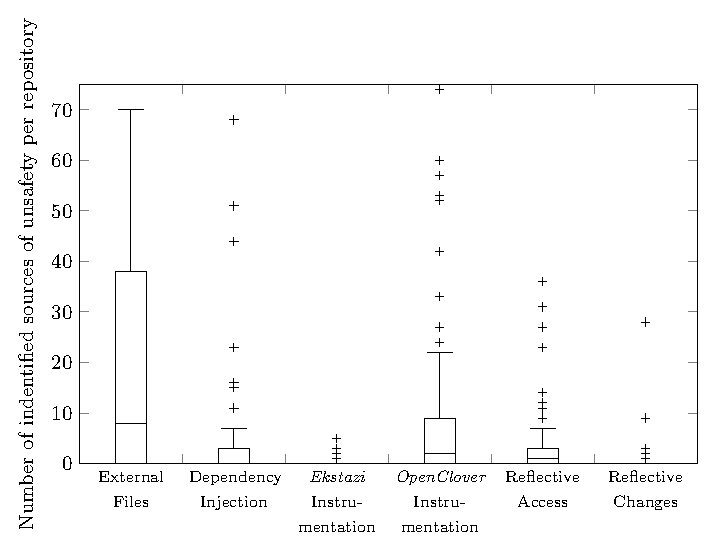
\includegraphics[scale=0.9]{./figures/pdf/box_plot.pdf}
\end{figure}

Figure~\ref{fig:probs_commits} visualizes the composition of sources of unsafety on a commit-level.
Unsafety produced by runtime instrumentation is not included in the graphic. It is
not caused by changes introduced in a commit, but by the underlying code base that contains the
problematic method calls. We also only recorded all appearances of the \texttt{Class.forName(...)}
method call for every commit without explicitly documenting the changes between commits. We used
this data to infer changes between commits, which also means that we do not have change data for
the first scanned commit of every repository.

\begin{figure}[h]
    \caption{Absolute number of commits that contain the associated source of unsafety (over all projects).}\label{fig:probs_commits}
    \centering
    \vspace{2em}
    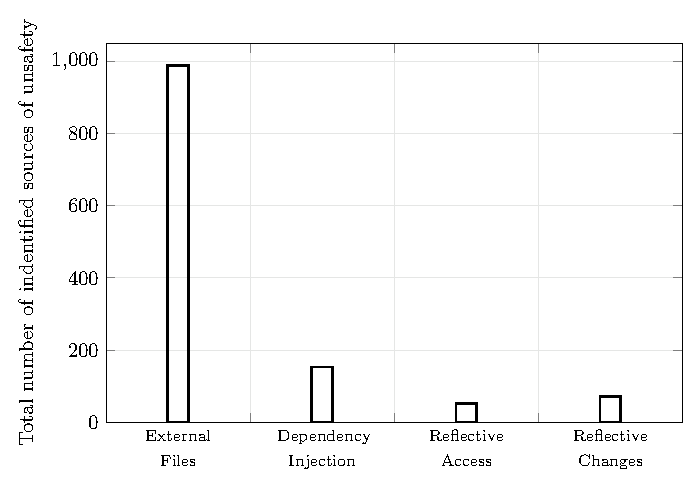
\includegraphics[scale=0.7]{./figures/pdf/commit_bar.pdf}
\end{figure}

\subsubsection{External Files}
With this scanner, we identified a total of $989$ commits that change an average of
$11.85$ external files in the searched paths. The commits change, on average, $1993.59$ lines of
text in the external files. This number only includes changes on external files whose content is
versioned via git. Even though most of these file changes may not change the program's behavior,
they all are sources of unsafety, because their changes are not detected by most of the examined
\ac{rts} tools.

\subsubsection{\acf{di}}
Of the $100$ examined projects, $53$ depend on libraries from the Spring framework, $17$ on Guice
libraries, $5$ on the CDI \ac{di} implementation and $3$ on the Dagger \ac{di} framework. This shows
that \ac{di} is an important factor in evaluating the unsafety of \ac{rts}-tools.

For in-depth scans, we concentrated on Spring and Guice \ac{di} features. We recorded $484$ changes on
Spring-related and $297$ changes on Guice-related keywords (listed in
Table~\ref{table:dep_inj_keywords}). None of the examined repositories uses Guice in combination with the
Netflix Governator library that allows for automatic classpath scanning.

\subsubsection{Runtime Instrumentation}
This scanner identified $63$ programs whose behavior changes due to the
profiling and coverage approaches used by \emph{Ekstazi} and \emph{OpenClover}. $11$ repositories
contain code that cannot be executed with \emph{Ekstazi}'s runtime instrumentation enabled. 
\emph{OpenClover} changes the behavior of
code in $49$ repositories. $3$ projects contain code that is affected by both tools. 
With, on average, $14.80$ incompatible files per
affected repository, this source of unsafety normally renders the corresponding tool unusable for
the project. Though, if the repository still uses the tool, the resulting differences in test
results can cause correctly failing tests to pass and vice versa.

\subsubsection{Reflections}
We mainly scanned for appearances of the \texttt{Class.forName(...)} method call
that is the main reason for most reflection-related unsafety. Other methods of reference to meta
class instances require a static method call on the class that creates a solid dependency. $56$
of the projects use this method at least once, but in general between $1$ and $36$ times. We counted
$333$ occurrences across all repositories. In addition to this search, we also tried to follow the
loaded class paths and detect changes on these classes that loaded via reflections. The problems
with this approach are described in Section~\ref{scanner:reflections}. We were able to
detect a total of $72$ changes on classes that are loaded via reflections in $8$ projects. These
changes are undetected by \emph{STARTS} and \emph{HyRTS}. Their
static initialization is also undetected by all examined tools, making them a major, so far
undocumented source of unsafety.

% Things to note:
% - Commit hashes are excepted to be unique among all projects
% - Runtime instrumentation was only recorded project wide and is therefore not respected for commit-level analysis
% - Reflection access was also only recorded on a project level but was calculated back to changes -> missing changes from first commit!
% - Of the 10000 commits, 1151 commits introduced unsafe behavior (runtime instrumentation ignored) -> 11.51\%
% How many projects are free of detected unsafety? Which projects contain all sources of unsafety?

\section{Discussion}
\subsubsection{Maintenance}
Many of the problems and sources of unsafety introduced by the examined \ac{rts}-tools are caused by
incompatibilities of the tools with modern language features. Especially \emph{Ekstazi}, being one of the
most promising examined tools, is outdated and cannot be used in projects in its current state.
This abandonment of \ac{rts}-tools, such as \emph{HyRTS}, \emph{Ekstazi} and \emph{GIBstazi}\footnote{\emph{STARTS} has recently
    been maintained and is therefore not considered abandoned.}, leads to a market full of
unusable \ac{rts} solutions. Research should focus more on updating and improving existing open
source solutions than developing new projects from scratch that are not going to be maintained.

\subsubsection{Usability of the Examined Tools}
Looking at the discovered sources of unsafety and their occurrence in current Java software development,
it is clear that none of the examined tools should be used without in-depth knowledge of their
downsides. Because of the continued maintenance on the \emph{STARTS} program, we see high future potential in
this static \ac{rts}-tool. However, the current latest official release (version 1.3) is not functional. The
previously described state of dynamic \ac{rts} for Java is alarming. The examined tools are all
poorly maintained. The most up-to-date tool is \emph{OpenClover} with its last release in October 2019.
The dynamic tools also act surprisingly unsafe, compared to the possibilities they have for monitoring changes.

\subsection{Limitations}
This paper does not claim to include all sources of unsafety that occur when using one of the
examined tools. They may contain bugs that we did not find. Other external tools or libraries, for example other
\ac{di} frameworks than Spring or Guice, could also cause undiscovered unsafety. We concentrated on
evaluating the major causes of unsafety that are likely to occur in real world software projects.

The results of the repository scanning are limited by the number of scanner modules, our methodology
and the selection of projects. We did not scan for all discovered sources of unsafety. Our scanning
approach trades simplicity for accuracy, meaning the results are prone to including false positives
and false negatives.
Every line of text in a Java source code file was treated as runnable code, only plaintext files
were analyzed. Many well known Java projects were excluded from this study, because we use the GitHub stars
feature to determine the popularity of projects and they did not have enough stars to be included in
the top 100 repositories.

We excluded all projects that do not use the Maven build system. This was necessary to enforce a
uniform project structure for the external files scanner module. The Maven tool is used by
approximately 60\% of all Java projects~\cite{project_management_tools_report}, making it a viable prerequisite for scanned projects. 

\section{Threads to Validity}

\subsubsection{External}
The examined study objects are a selection of currently available \ac{rts}-tools for the Java
programming language that may not fully represent the capabilities and problems of other existing
tools. We chose this selection of promising static and dynamic \ac{rts} solutions based on their
occurrence in other studies and software projects. The repository selection of the 100 projects 
that were scanned may also limit the generalizability of the results. For this reason, we have chosen the
repositories base on their popularity and not based on other research papers or external sources,
like it was done in previous research~\cite{ekstazimain,hyrts_paper,starts_paper}. 
% Selecting only
% repositories that use Maven for project management might have introduced a slight selection bias,
% but was necessary 

\subsubsection{Internal}
\ac{poc} repositories and automatic scan scripts may contain bugs. To mitigate this risk, we
performed tests on \ac{poc} repositories manually and multiple times to identify flaky and buggy behavior.
The code for the evaluation of scan results was written twice in different ways to eliminate logical
programming errors. We only used well maintained, popular open source libraries for the git integration
and data manipulation to reduce the risk of hidden errors in third party code.

\section{Conclusions}\label{sec:conclusion}

The presented evidence uncovers the alarming situation of safe \ac{rts}-tools for Java. Through a
combination of incompatibilities with new language features, methodological limitations and
implementation errors, the examined \ac{rts} solutions are
prone to act in an unsafe manner. The latest versions of the examined tools are all not safely usable in software
projects. Further research is required not to create new, supposedly safe \ac{rts}-tools that end up like our study objects,
but to update the most promising solutions and eliminate existing bugs. An up-to-date open source
implementation of safe \ac{rts} for Java will show that \ac{rts} is achievable and
has great potential for saving time and processing resources, without compromising regression test safety.

%
% ---- Appendix ----
%
\appendix
\section{Appendix}\label{sec:appendix}

\begin{table}[H]
    \caption{Keywords required for unsafety in dependency injection.}\label{table:dep_inj_keywords}
    \centering
    \begin{tabular}{l | l || l | l}
        \hline
        \multicolumn{2}{l ||}{Spring Framework} & \multicolumn{2}{| l}{Guice Framework}                                                                   \\
        \hline
        Keyword                                & Regular expression                    & Keyword                        & Regular expression             \\
        \hline
        \texttt{@Bean}                         & \texttt{@Bean}                        & \texttt{@AutoBindSingleton}    & \texttt{@AutoBindSingleton}    \\
        \texttt{@Component}                    & \texttt{@Component}                   & \texttt{@Provides}             & \texttt{@Provides}             \\
                                               &                                       & \texttt{@CheckedProvides}      & \texttt{@CheckedProvides}      \\
                                               &                                       & \texttt{@ProvidesIntoSet}      & \texttt{@ProvidesIntoSet}      \\
                                               &                                       & \texttt{@ProvidesIntoMap}      & \texttt{@ProvidesIntoMap}      \\
                                               &                                       & \texttt{@ProvidesIntoOptional} & \texttt{@ProvidesIntoOptional} \\
                                               &                                       & \texttt{bind(...)}             & \verb|bind\(.*\)|         \\
                                               &                                       & \texttt{LifecycleInjector}     & \texttt{LifecycleInjector}     \\
    \end{tabular}
\end{table}

\vspace{1cm}

\begin{table}[H]
    \caption{Methods whose behavior changes with the corresponding \ac{rts}-tools runtime
        instrumentation. All methods are called on the meta class object of type \nolinkurl{Class}.}\label{table:runtime_instr_methods}
    \centering
    \begin{tabular}{l | l}
        \hline
        \emph{Ekstazi}                    & \emph{OpenClover}             \\
        \hline
        \texttt{getAnnotatedInterfaces()} & \texttt{getDeclaredClasses()} \\
        \texttt{etAnnotatedSuperclass()}  & \texttt{getDeclaredFields()}  \\
        \texttt{toGenericString()}        & \texttt{getClasses()}         \\
                                          & \texttt{getFields()}          \\
    \end{tabular}
\end{table}

\vspace{1cm}

\begin{figure}[H]
    \caption{Sources of unsafety per repository, discovered in repositories and commits collected in
        Section~\ref{sec:foss_search} (Including all outliers).}\label{appx:fig:box_plot}
    \centering
    \vspace{2em}
    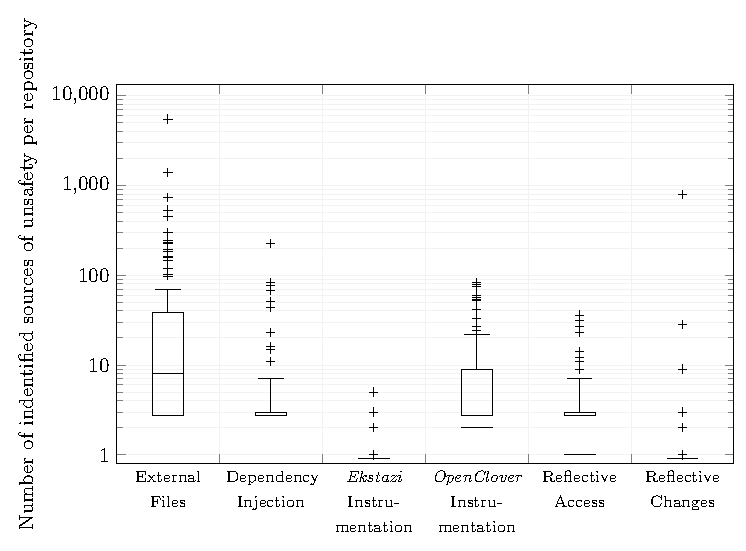
\includegraphics{./figures/pdf/box_plot_outliers.pdf}
\end{figure}

\vspace{1cm}

\begin{longtable}{l | l | l | l}
    \caption{List of selected open source projects. (Collected between 11/11/2021 and 11/13/2021)}\label{table:foss_projects_list}                  \\
    \hline
    Organisation / User & Repository Name           & Stars & \parbox[l][4.2em][c]{7em}{Last examined \\commit hash\\(truncated)} \\
    \hline
    \endfirsthead
    \hline
    Organisation / User & Repository Name           & Stars & \parbox[l][4.2em][c]{7em}{Last examined \\commit hash\\(truncated)} \\
    \hline
    \endhead
    iluwatar            & java-design-patterns      & 71106 & 2674cb9523a6                            \\
    google              & guava                     & 42835 & a2bbcc3bc2b4                            \\
    apache              & dubbo                     & 36435 & ae6c6a9a9ab1                            \\
    zxing               & zxing                     & 28624 & c25029d29ad2                            \\
    eugenp              & tutorials                 & 28091 & 41c8af76d2c9                            \\
    netty               & netty                     & 27936 & 3d6bed01cd07                            \\
    alibaba             & arthas                    & 27624 & 3792ca308785                            \\
    apolloconfig        & apollo                    & 25882 & 02fff624870a                            \\
    alibaba             & druid                     & 24749 & 3b4e77034a62                            \\
    xkcoding            & spring-boot-demo          & 23941 & f10dc0a45be8                            \\
    alibaba             & fastjson                  & 23926 & 869746101f6d                            \\
    dbeaver             & dbeaver                   & 23148 & 2e1a4eda8b07                            \\
    alibaba             & easyexcel                 & 21750 & f8fd5f0427f0                            \\
    alibaba             & canal                     & 21143 & b54bea5e3337                            \\
    seata               & seata                     & 21111 & 5ddfbc1f3cb7                            \\
    alibaba             & spring-cloud-alibaba      & 20593 & 8bd5a8d688d4                            \\
    alibaba             & nacos                     & 20257 & 5a4d433970be                            \\
    google              & gson                      & 20255 & 6e06bf0d89ad                            \\
    apache              & skywalking                & 18107 & b63008c61e1f                            \\
    jenkinsci           & jenkins                   & 18057 & 09f0269e8762                            \\
    alibaba             & Sentinel                  & 17814 & 0a34fc4d1139                            \\
    redisson            & redisson                  & 17747 & fdcb943828c5                            \\
    apache              & flink                     & 17519 & 1529b78ddc4a                            \\
    mybatis             & mybatis-3                 & 16455 & a2cdac6f7664                            \\
    brettwooldridge     & HikariCP                  & 15981 & 8b4a6bbebb77                            \\
    apache              & rocketmq                  & 15852 & df4e98855d46                            \\
    openzipkin          & zipkin                    & 14868 & b6a5f76c4d13                            \\
    apache              & shardingsphere            & 14825 & c2c51985437e                            \\
    prestodb            & presto                    & 12808 & 70f8f59e0889                            \\
    eclipse-vertx       & vert.x                    & 12482 & 3c494da0a4a8                            \\
    YunaiV              & SpringBoot-Labs           & 12249 & 85c7322b9d1a                            \\
    eclipse             & deeplearning4j            & 12244 & a12d6eecbc61                            \\
    apache              & hadoop                    & 12081 & 7bc78ab70790                            \\
    pinpoint-apm        & pinpoint                  & 11801 & 15577df66448                            \\
    apache              & druid                     & 11335 & 6f6e88e02ed0                            \\
    pagehelper          & Mybatis-PageHelper        & 10763 & 4b0484662bae                            \\
    google              & guice                     & 10532 & 0ce94279a16d                            \\
    keycloak            & keycloak                  & 10508 & 2f8c5dd05e74                            \\
    thingsboard         & thingsboard               & 10358 & f2974532c607                            \\
    codecentric         & spring-boot-admin         & 10331 & 2076c6ac1d85                            \\
    OpenAPITools        & openapi-generator         & 10276 & 70737fb1e6b6                            \\
    redis               & jedis                     & 10127 & 253664ff1eac                            \\
    apache              & zookeeper                 & 9962  & 864b8a7c8044                            \\
    apache              & pulsar                    & 9880  & 2c4d913c4b3f                            \\
    square              & javapoet                  & 9255  & 88517888277e                            \\
    perwendel           & spark                     & 9209  & 54079b0f95f0                            \\
    MyCATApache         & Mycat-Server              & 9140  & 92174cd734f1                            \\
    jhy                 & jsoup                     & 9122  & 46b0b9569a76                            \\
    quarkusio           & quarkus                   & 8816  & 0f896210478b                            \\
    TooTallNate         & Java-WebSocket            & 8558  & bcfc9675d611                            \\
    OpenRefine          & OpenRefine                & 8481  & 8d06810af85a                            \\
    stanfordnlp         & CoreNLP                   & 8219  & 0f7c464edc7c                            \\
    junit-team          & junit4                    & 8213  & 7167b23b3ba7                            \\
    Activiti            & Activiti                  & 8159  & f9351cc5b978                            \\
    dropwizard          & dropwizard                & 8054  & 684c51ecbf43                            \\
    square              & moshi                     & 7744  & 954ca46b9ed9                            \\
    OpenFeign           & feign                     & 7607  & f21d32a7d9d9                            \\
    apache              & shardingsphere-elasticjob & 7320  & 49506b53cbfa                            \\
    signalapp           & Signal-Server             & 7210  & aaa2a6eef17f                            \\
    vipshop             & vjtools                   & 7182  & 4c1ee2a312b7                            \\
    questdb             & questdb                   & 6915  & 883474bd7513                            \\
    alibaba             & otter                     & 6893  & 7f80d17d74e5                            \\
    apache              & dolphinscheduler          & 6702  & daf21b09dd94                            \\
    abel533             & Mapper                    & 6658  & 84e33f7c9e11                            \\
    NLPchina            & elasticsearch-sql         & 6539  & 4b1c87eb1cfe                            \\
    Angel-ML            & angel                     & 6437  & 0e60cddf5efa                            \\
    checkstyle          & checkstyle                & 6337  & b6e54419d8bd                            \\
    apache              & storm                     & 6297  & f481eaf043db                            \\
    NanoHttpd           & nanohttpd                 & 6118  & efb2ebf85a2b                            \\
    Graylog2            & graylog2-server           & 5890  & 4ddbc427df79                            \\
    AsyncHttpClient     & async-http-client         & 5854  & c959fa0483ad                            \\
    google              & error-prone               & 5749  & f10bba5891d9                            \\
    weibocom            & motan                     & 5746  & f9c46071eafc                            \\
    sohutv              & cachecloud                & 5674  & f9dfc98eadcf                            \\
    debezium            & debezium                  & 5625  & 39ecc4e73248                            \\
    joelittlejohn       & jsonschema2pojo           & 5608  & 4d00331095a1                            \\
    rest-assured        & rest-assured              & 5584  & 4eeb3d82b1d4                            \\
    lets-blade          & blade                     & 5563  & 118d856b53bd                            \\
    languagetool-org    & languagetool              & 5535  & a76e5ab4938c                            \\
    apache              & zeppelin                  & 5478  & cd09f93b0d71                            \\
    apache              & incubator-shenyu          & 5463  & 2f5cc73fb7f5                            \\
    karatelabs          & karate                    & 5383  & 14807dbf8d7c                            \\
    pentaho             & pentaho-kettle            & 5336  & b79362de3e19                            \\
    Alluxio             & alluxio                   & 5300  & b9681d4ec598                            \\
    scribejava          & scribejava                & 5218  & 124745961e99                            \\
    JodaOrg             & joda-time                 & 4723  & e9337f0c0955                            \\
    quartz-scheduler    & quartz                    & 4706  & cbce9b6d0669                            \\
    hazelcast           & hazelcast                 & 4611  & d05be9ecf18d                            \\
    raphw               & byte-buddy                & 4601  & 7402e597870d                            \\
    confluentinc        & ksql                      & 4598  & 0de5dda35ccc                            \\
    mapstruct           & mapstruct                 & 4567  & 735a5bef6a36                            \\
    flowable            & flowable-engine           & 4562  & f7323c2b0424                            \\
    gephi               & gephi                     & 4503  & db454c59cc9d                            \\
    spring-projects     & spring-security-oauth     & 4484  & 2b58aafecac3                            \\
    spring-cloud        & spring-cloud-netflix      & 4483  & dc45b7f580fa                            \\
    sofastack           & sofa-boot                 & 4405  & f65941f97fb9                            \\
    orientechnologies   & orientdb                  & 4378  & 3a394ef87dc4                            \\
    trinodb             & trino                     & 4368  & a836e7c223b1                            \\
    lettuce-io          & lettuce-core              & 4262  & b0a392f606d9                            \\
    apache              & hbase                     & 4260  & 8458e44a1a7d                            \\
\end{longtable}

%
% ---- Bibliography ----
%
\clearpage
\bibliographystyle{splncs04}
\bibliography{library.bib}
%
\clearpage
\vspace*{\fill}
\doclicenseThis
\end{document}


% TODO:
% - Tenses?
% - we too much?
% - Cite paper that evaluates starts, ekstazi and openclover and finds bugs in related work!
% - comparison of the tools, where? 
% - inline code
% - hyrts implementation missing -> super hard to find stuff -> security by obscurity.
% - Java 8 vs 1.8?
